\documentclass{book}

\usepackage{kavya-book}


\begin{document}
%-----------------------------------
% For customised Title Page
\thispagestyle{empty}
%\input{./title.tex} %Cover page
\thispagestyle{empty}
%\input{./inner.tex}	%Inner title page
%--------------------------------------------------------------------

%Default Title page 
\title{An eSim Guide \\ for \\ Electronic Circuit Simulation}
%\date{December 2013}
\author{Kavya Manohar} {%Authors: Kavya Manohar}
\maketitle
%----------------------------------------------------------
\chapter*{Copyright \textcopyright{}2015}
%\textbf{Copyright  }
  

%\\[2cm]
\noindent This work is licensed under a Creative Commons Attribution-Share Alike 4.0 India License. See \url{http://creativecommons.org/licenses/by-sa/4.0/} for more details.




%------------------------------------------------------------

\clearpage
\thispagestyle{plain}
%\par\vspace*{.35\textheight}{\centering Dedicated to my parents\par}  % code for dedication page
\chapter*{Acknowledgements}

This is a work-in-progress version of a beginner's guide for designing and simulating electronic circuits using open source tools - gEDA and Ngspice .

\paragraph{}
	This work would not have been possible without the documentations and tutorials acknowledged below:

\begin{itemize}
\item
gEDA user manual \url{http://wiki.geda-project.org/geda:gschem_ug}
\item
Ngspice home page \url{http://ngspice.sourceforge.net/}
\item
Ashwith's tutorials \url{http://ashwith.wordpress.com/tag/ngspice/}
\item
Circuit Simulation using gEDA and SPICE   \url{http://www.brorson.com/gEDA/SPICE/intro.html}
\end{itemize}

Thanks are in advance to every reader who is going to find this work useful. Your feed back is most welcome.

\flushright{Kavya Manohar}
\chapter*{Preface}

This is a quick guide for designing and simulating electronic circuits using open source  EDA tool- eSim. 
\paragraph{}

eSim is an open source EDA tool for circuit design, simulation, analysis and PCB design, developed by FOSSEE team at IIT Bombay. It is an integrated tool build using open source software such as Kicad (\url{http://www.kicad-pcd.org}), Ngspice (\url{http://ngspice.sourcefouge.net/}) It is released under GNU GPL License. It runs on Ubuntu Linux, Windows XP and Windows.

\paragraph{}
This guide assumes the readers are familar with the workflow of eSim and provides the solution to specific simulation problems. Hence new users of eSim are requested to have a read on esim user manual before using this guide for simulation.

\flushright{Kavya Manohar}





\thispagestyle{empty}
\tableofcontents
\thispagestyle{empty}
\thispagestyle{empty}

\listoffigures
\thispagestyle{empty}
%CHAPTER-----------------------------------------------------------------------

\chapter{Introduction}
\chapter{Diode Characteristics}

\subsection*{AIM}
\paragraph{}To design and implement a circuit for simulating the V-I characteristics of a diode.

\subsection*{DESIGN AND CIRCUIT DIAGRAM}
\paragraph{}

Inorder to draw the diode characteristics, we have to use a DC source of voltage which may be varied during simulation. The diode in the circuit should be associated with a coresponding `Diode model' during  simulations. As in a hardware circuits lab, a curernt limiting resistor may also be used in series with the diode and the DC source. The resulting circuit diagram is shown in the Figure \ref{diodeckt}  below:
\begin{figure}[h]
\centering
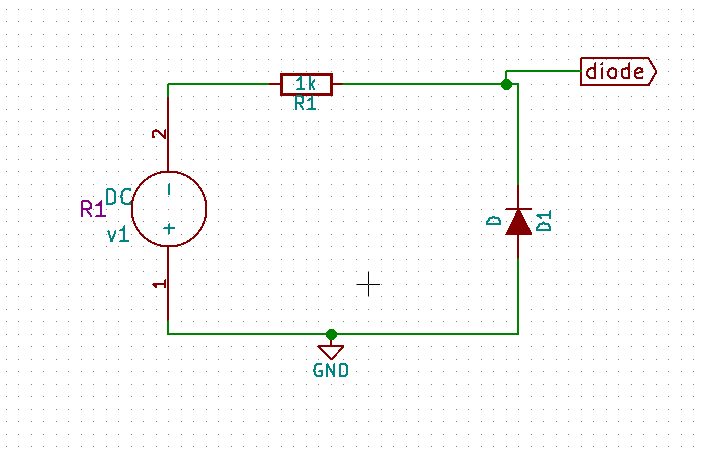
\includegraphics[width=0.8\textwidth]{diodeckt.png}
\caption{Schematic diagram for diode characteristics}
\label{diodeckt}
\end{figure}

\subsection*{PROCEDURE}

\subsubsection{Launch eSim}

\paragraph{}
 Launching eSim will take you to the dialog box which asks for the default workspace. Browsw the folders and set the wokspace location. It will finally end up in the eSim window shown in Figure \ref{LaunchWindow}.
\begin{figure}[h]
\centering
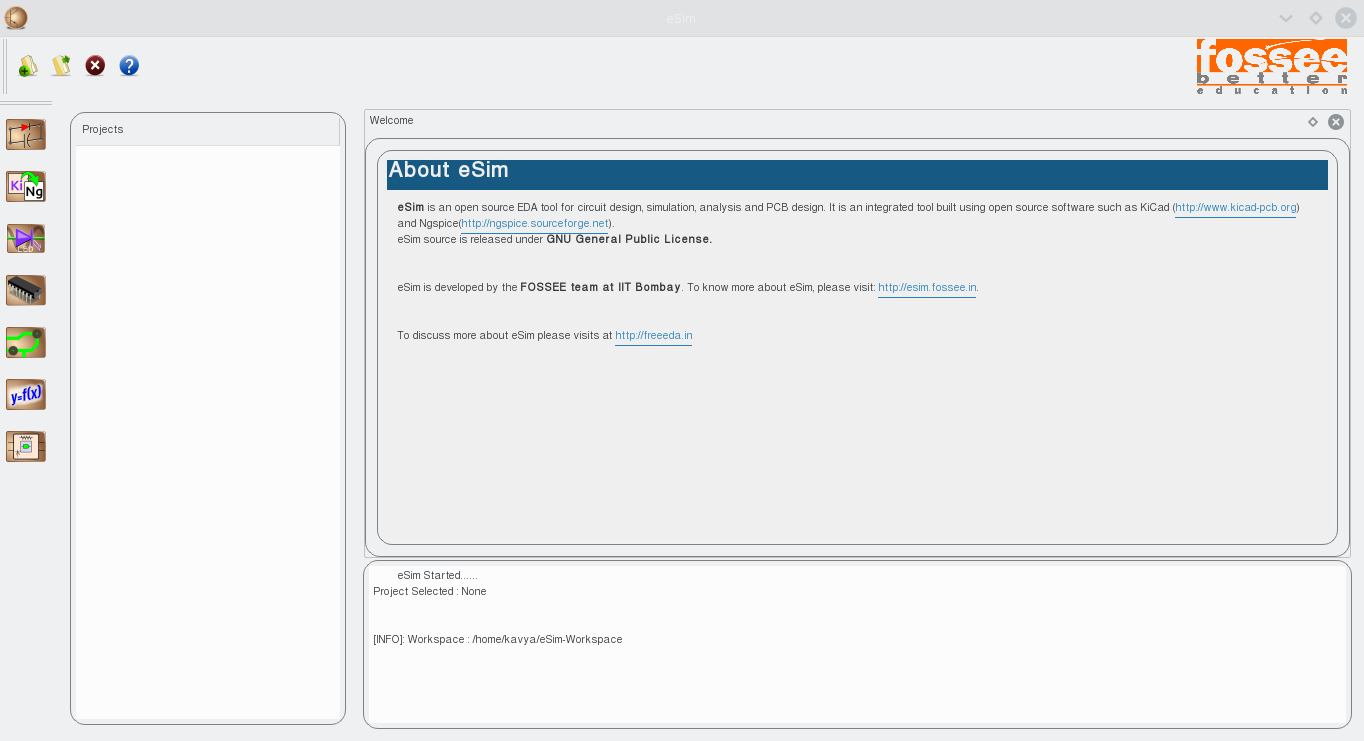
\includegraphics[width=0.8\textwidth]{LaunchWindow.png}
\caption{Launching eSim will take you to this window}
\label{LaunchWindow}
\end{figure}

\subsubsection{Create a New Project}

\paragraph{ } The new project is created by clicking the New icon on the
menubar. The name of the project is given in the pop up window as shown in Figure.\ref{newproject}.
\begin{figure}[h]
\centering
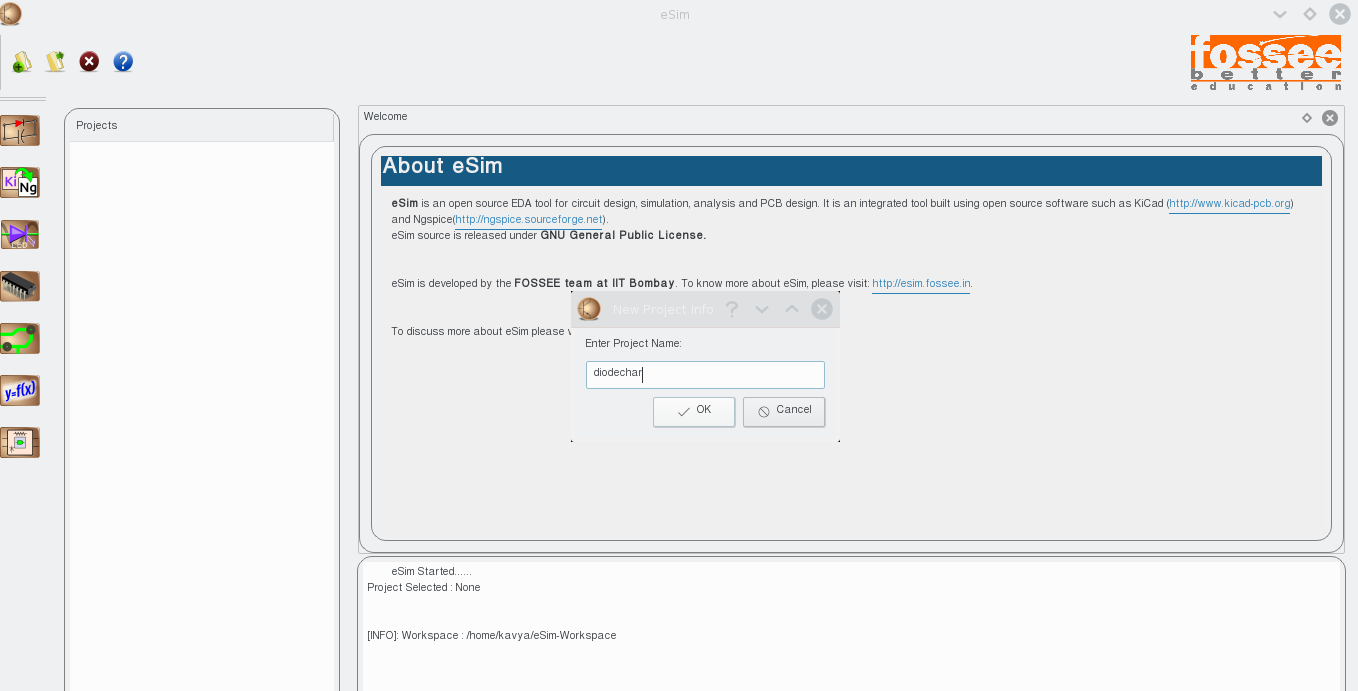
\includegraphics[width=\textwidth]{newproject.png}
\caption{Creating new project}
\label{newproject}
\end{figure}

\subsubsection{Create the Schematic}

\paragraph{}  To create the schematic, click the very first icon of the
left toolbar as shown in the Figure \ref{newschematic} .This will open KiCad Eeschema.


\begin{figure}[h]
\centering
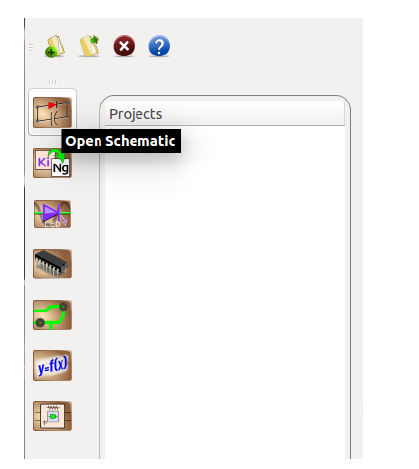
\includegraphics[width=0.5\textwidth, height=6cm]{newschematic.png}
\caption{Creating new schematic diagram}
\label{newschematic}
\end{figure}

To create a schematic in KiCad, we need to place the required components. See Figure \ref{kicad}

\begin{figure}[h]
\centering
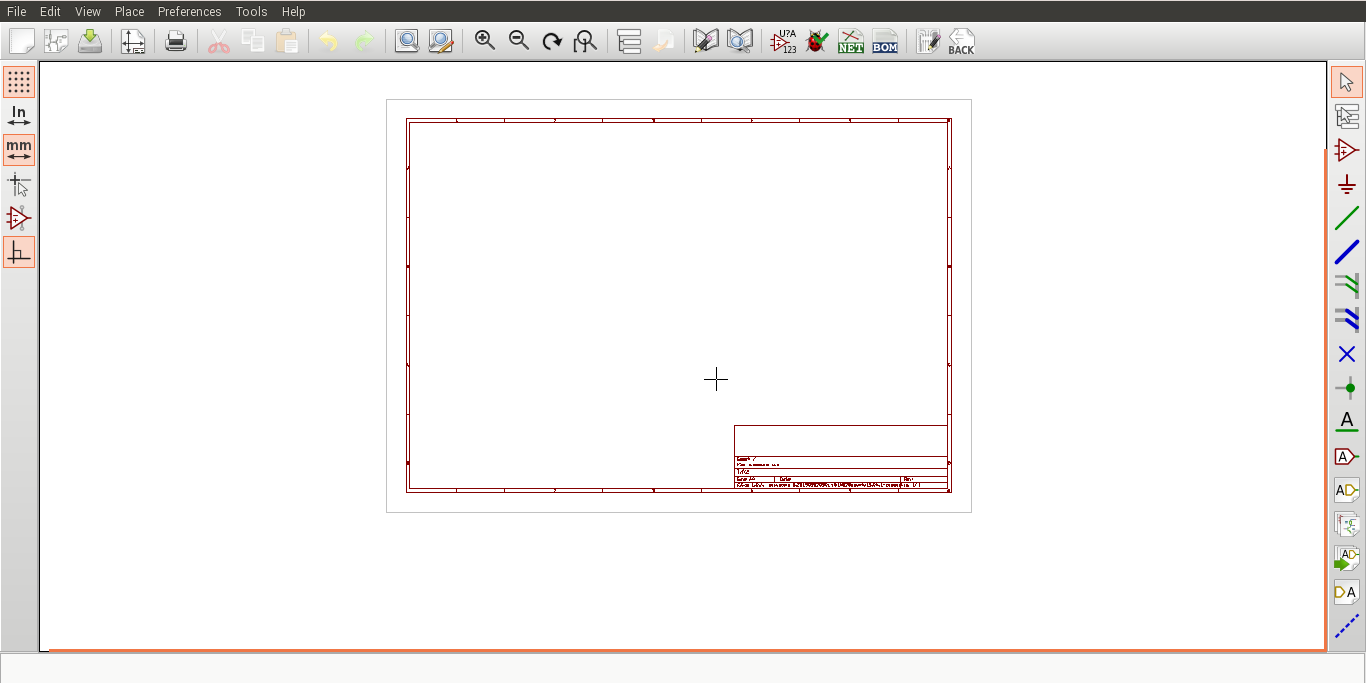
\includegraphics[width=0.5\textwidth, height=6cm]{kicad.png}
\caption{The Kicad Eeschema page}
\label{kicad}
\end{figure}

 Figure \ref{placecomponent}
shows the icon on the right toolbar which opens the component library. After all the required components of the simple RC circuit are placed, wiring is
done using the Place Wire option as shown in the Figure \ref{placewire}.Scroll up and down for zooming in and out.


\begin{figure}
\begin{minipage}{.5\textwidth}
  \centering
  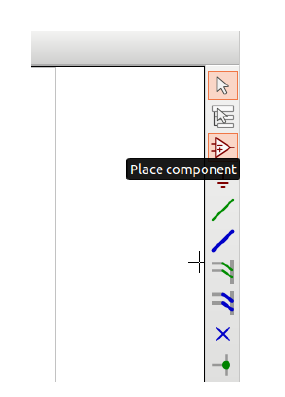
\includegraphics[width=\linewidth]{placecomponent.png}
  \caption{Place component icon}
  \label{placecomponent}
\end{minipage}%
\begin{minipage}{.5\textwidth}
  \centering
  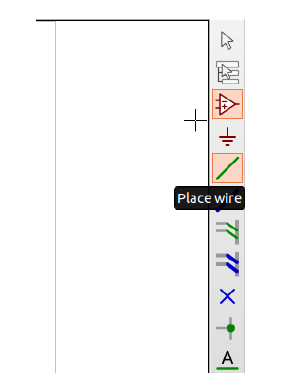
\includegraphics[width=\linewidth]{placewire.png}
  \caption{Place wire icon}
  \label{placewire}
\end{minipage}
\end{figure}


\paragraph{Placing the Components:} Normally all the components availbale in eSim can be chosen by left mouse click in the grid. The components are listed in different libraries. See Figure \ref{librarylist}.

\begin{figure}[h]
\centering
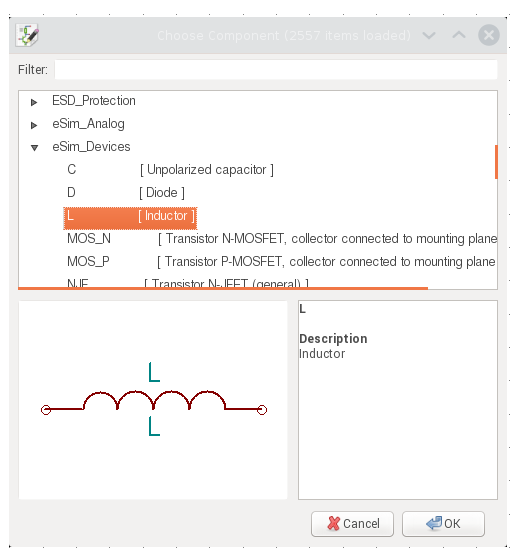
\includegraphics[width=0.5\textwidth, height=4cm]{librarylist.png}
\caption{The Kicad Libraries of components}
\label{librarylist}
\end{figure}

\begin{itemize}
\item
Choose DC source from eSim\_Sources
\item
Choose R from eSim\_Devices
\item
Choose D from eSim\_Devices
\item
Choose GND from power
\end{itemize}

Wire the components to get the circuit. A global label `diode' has been added to identify that node whose voltage will be later recorded and plotted.

\paragraph{Annotating the circuit:} Once the schematic diagram is completed, annotate it so that the `question marks' associated with the components are converted to meaningful numbers automatically. 
Select the resistor and edit its component value to 1k as shown in Figure \ref{editvalue}.

\begin{figure}[h]
\centering
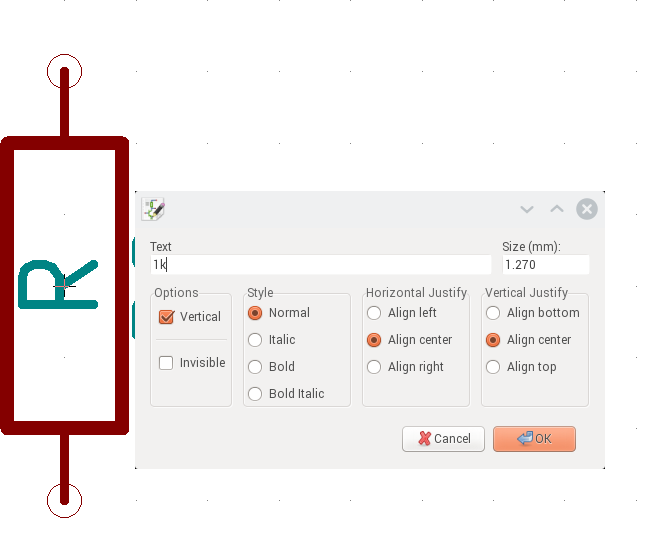
\includegraphics[width=0.5\textwidth, height=6cm]{editvalue.png}
\caption{Editing the value field of compenent R}
\label{editvalue}
\end{figure}

 Now we have the circuit diagram as shown in Figure \ref{diodeckt}.


\paragraph{Note:} If some libraries are found missing, you can add them from the `Preferences` menu by following the procedure: 

\begin{enumerate}
\item
Choose `Component Libraries' from Preferences menu.

\item
Click on the Add button on the top right side of the window.

\item
Choose the required libraries from `user/share/kicad/library' and click OK button

\end{enumerate}

\subsubsection{Create Netlist}




\begin{appendix}
%\input{chapters/referencedata.tex}
\end{appendix}
\begin{thebibliography}{1}

\bibitem{esimusermanual}{User Manual of eSim by FOSSEE, IIT Bombay.(\url{http://esim.fossee.in/resource/book/esimusermanual.pdf}}


\end{thebibliography}


\end{document}
